\setcounter{chapter}{5}
\chapter{Results}

Tentative layout: 


\section{Code development}

\begin{figure}
    \centering
    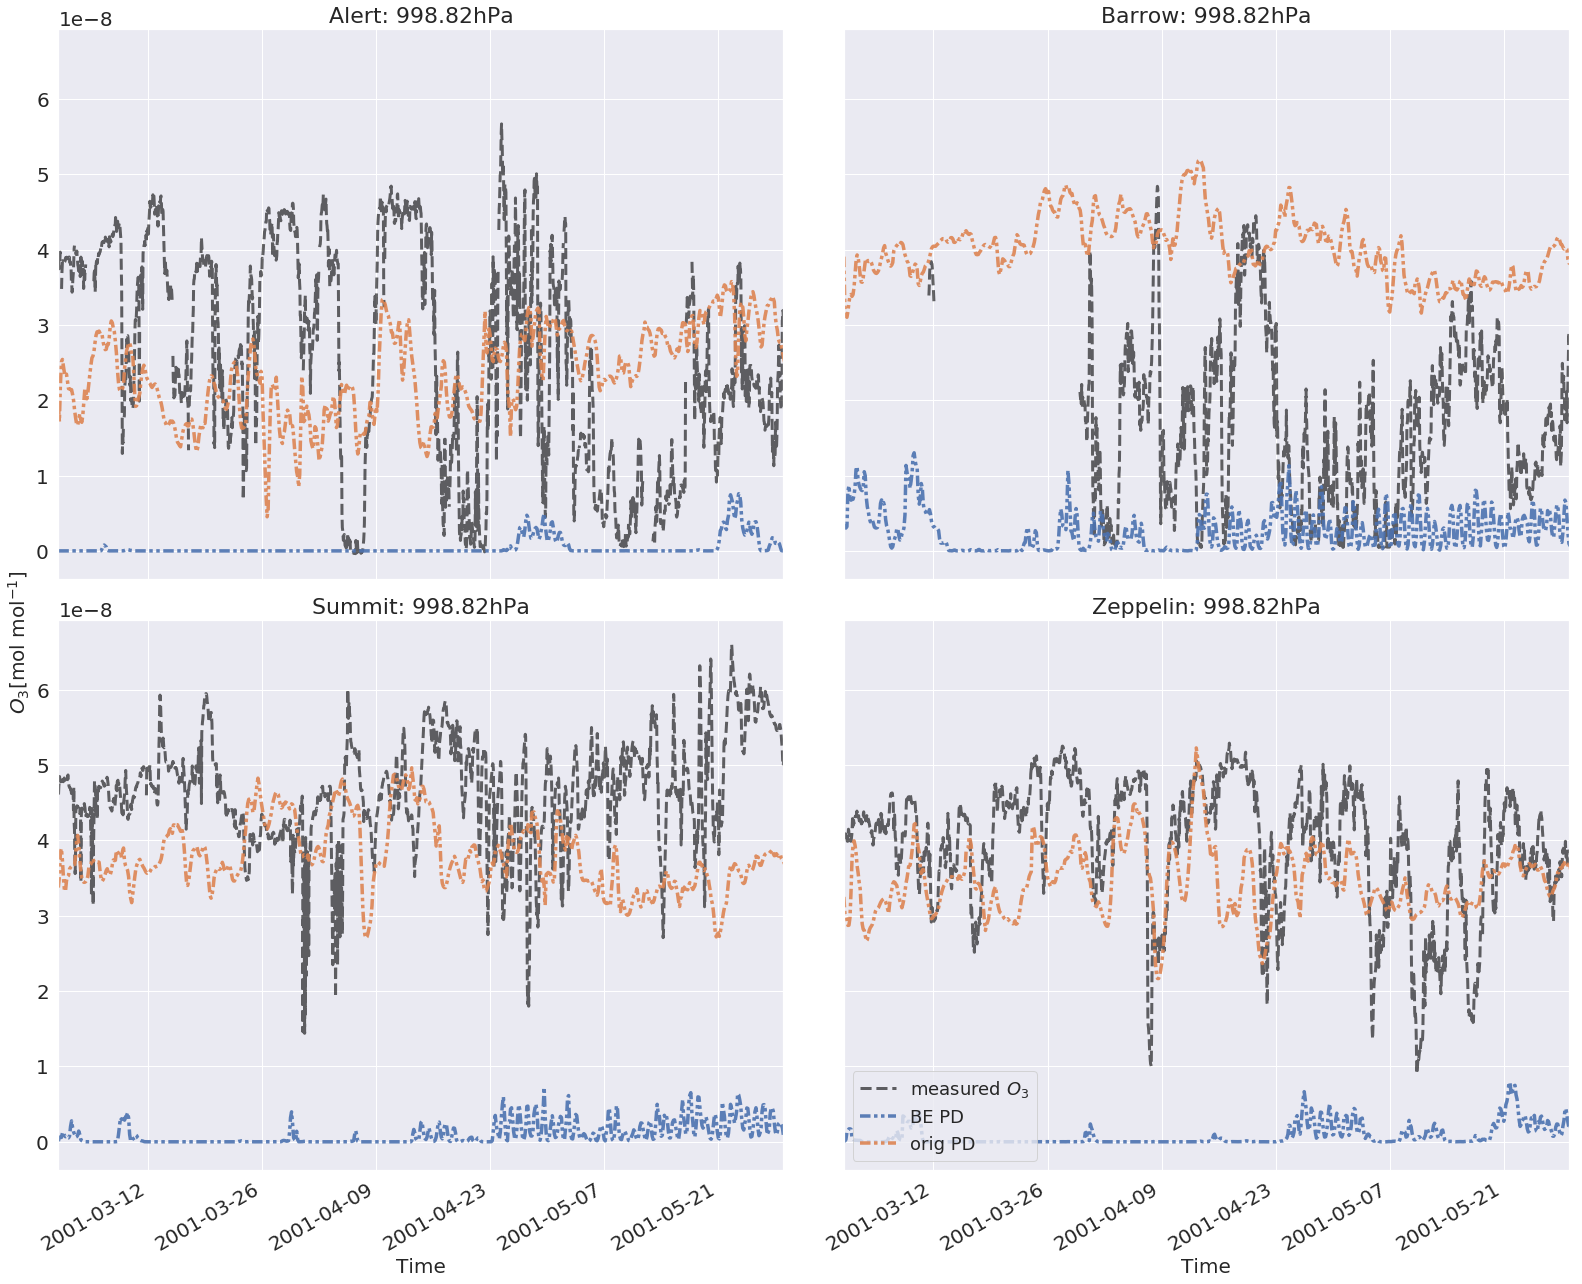
\includegraphics[width = \linewidth]{Chapter6_Results/images/ozone_2001_compObsOrigBE.png}
    \caption{Caption}
    \label{fig:CompObsOrigBE}
\end{figure}

\begin{figure}
    \centering
    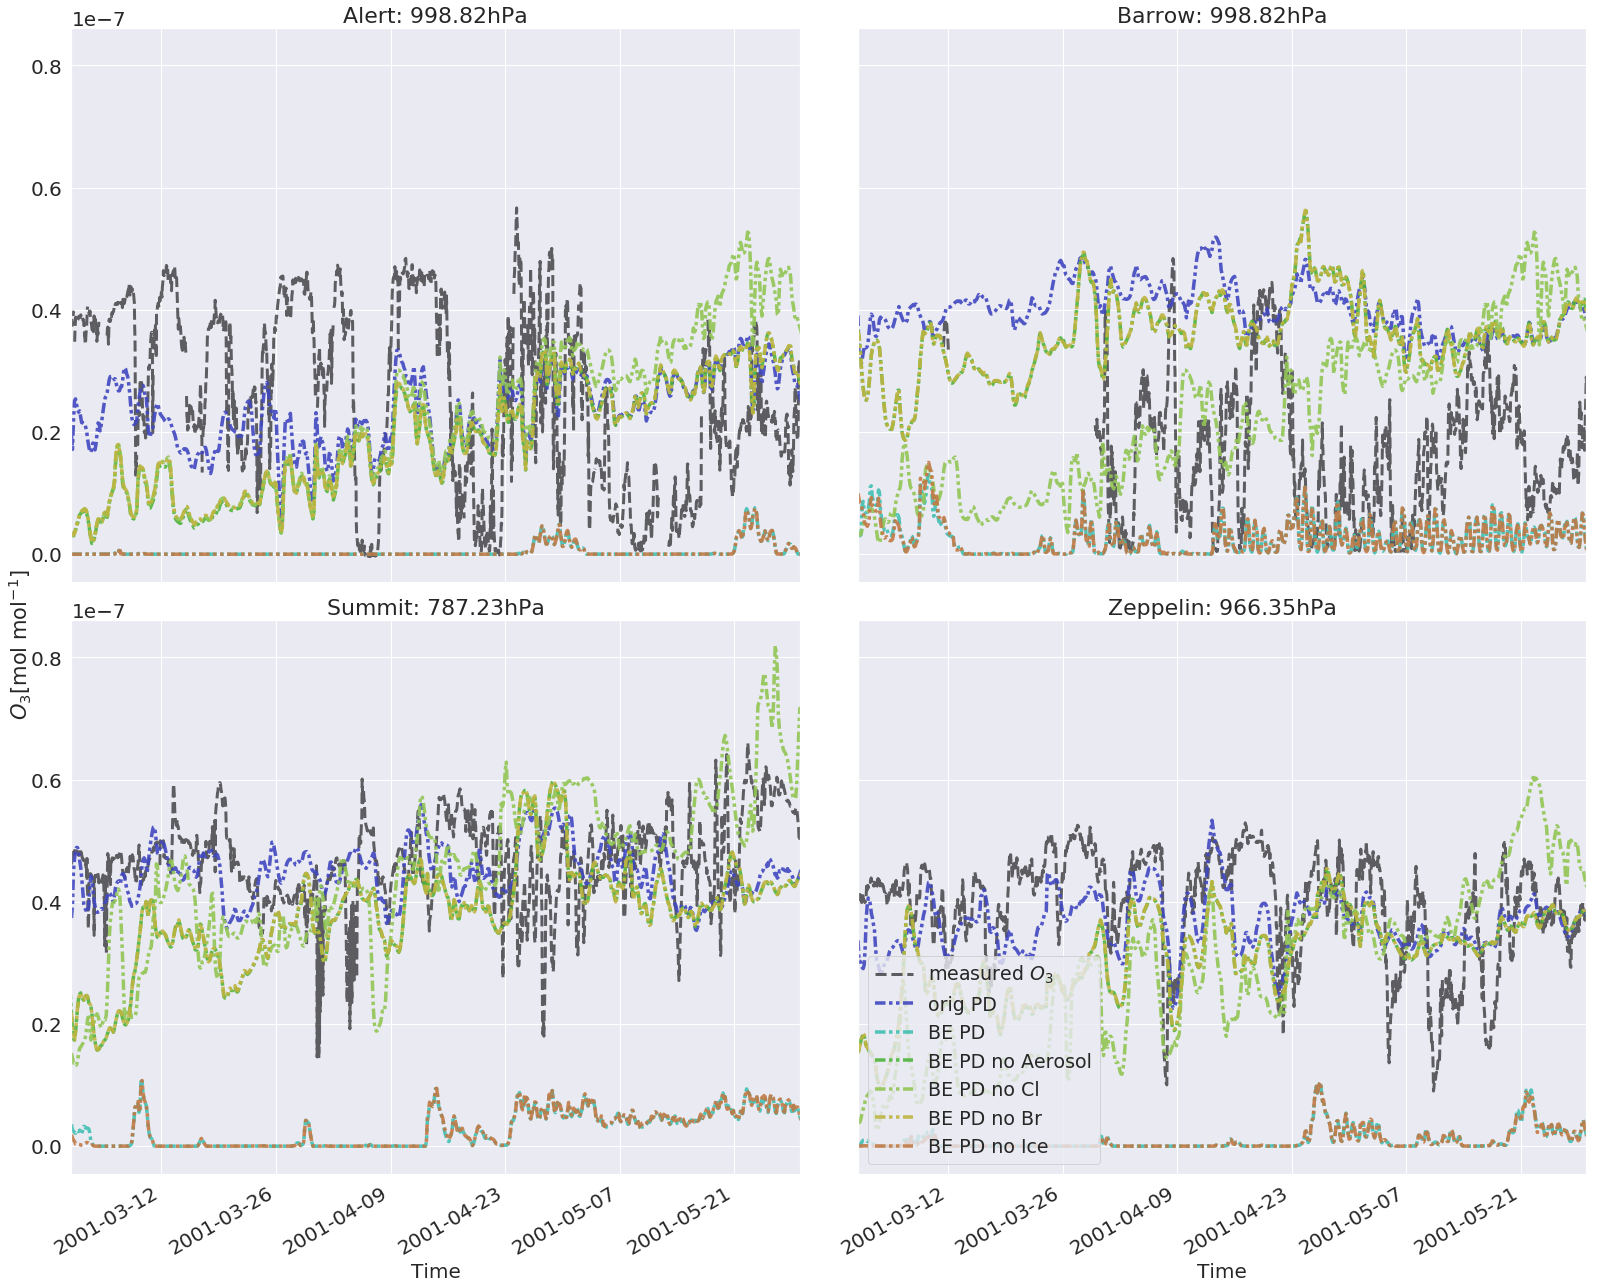
\includegraphics[width = \linewidth]{Chapter6_Results/images/ozone_removingHetReacts.png}
    \caption{Ozone measurements (black line) and model results from the original CTM3 (blue line), Branch \ref{def:BE_PD} (turquoise line), Branch \ref{def:BE_PD_noAerosol} (green line), \ref{def:BE_PD_noIce} (orange line), Branch \ref{def:BE_PD_noCl} (light green line) and Branch \ref{def:BE_PD_noBr} (yellow line) at the four different stations, Alert (top left), Barrow (top right), Summit (lower left) and Zeppelin (lower right) with available measurements in 2001. Model results were taken from the approximate altitude of the station in hPa. PD = present day, BE = bromine explosion}
    \label{fig:test_RemoveHetReacts}
\end{figure}

\begin{figure}
    \centering
    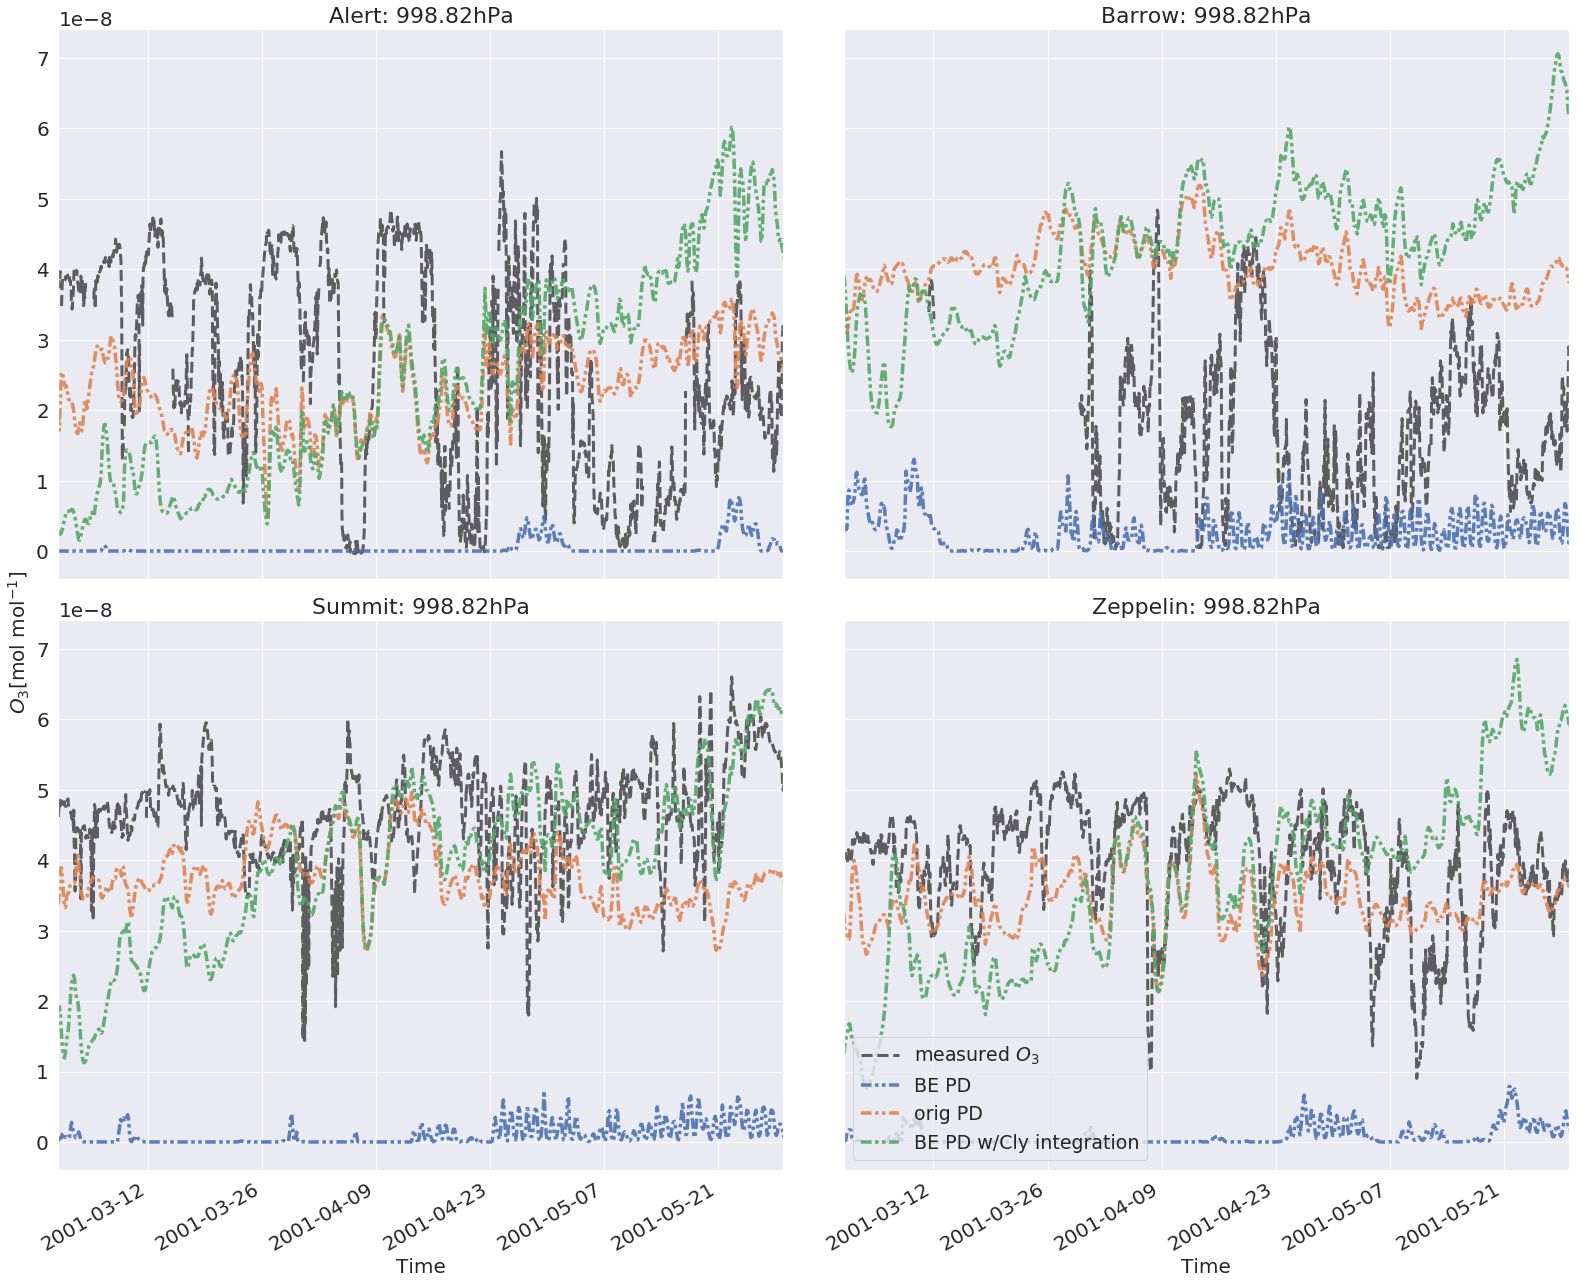
\includegraphics[width = \linewidth]{Chapter6_Results/images/ozone_2001_newClyIntegration.png}
    \caption{Ozone measurements (black line) and model results from the original CTM3 (orange line), Branch \ref{def:BE_PD} (blue line) and the attempt to integrate the $\chem{Cl_y}$ family (green line) at the four different stations, Alert (top left), Barrow (top right), Summit (lower left) and Zeppelin (lower right) with available measurements in 2001. Model results are taken from the first model level at $998.82 hPa$. PD = present day, BE = bromine explosion}
    \label{fig:test_ClyInt}
\end{figure}

\section{Comparison between the PD- and PI-branches}

\section{Comparison with station data}

\section{Comparison with literature}

Measurements of $\chem{Br_2}$, \chem{BrCl} and $\chem{O_3}$ were conducted by \cite{Foster2001} at Alert research station. They found $\chem{Br_2}$ mixing ratios up to $\sim$ 25 \acrshort{ppt} and \chem{BrCl} at mixing ratios up to 35 \acrshort{ppt} between day 40 and 75 in 2001. Ozone was depleted from background values of $\sim$ 30-40 \acrshort{ppb} to below 10 ppb. 

\medskip

\cite{Simpson2017} investigated the \chem{BrO} column using \acrlong{maxdoas} instrumentation near Barrow in 2012.

\medskip

\cite{Luo2018} also investigated the \chem{BrO} column using \acrshort{maxdoas} in Ny Ålesund in 2015. 

\medskip

\cite{Thomas2012} and \cite{Thomas2011} about the mechanism behind ODEs at Summit, Greenland. 

\section{Calculation of radiative forcing using PD- and PI model results}